%% ============================================================
%%  Chapter 7 – Pickup-and-Delivery Problems for People Transportation
%%  Vehicle Routing: Problems, Methods, and Applications, 2nd ed., 2014
%%  Authors of the chapter: Karl F. Doerner, Juan José Salazar-González
%% ============================================================
\documentclass[aspectratio=169,10pt]{beamer}

\usetheme{Madrid}
\usecolortheme{seahorse}

\usepackage{amsmath,amssymb,amsfonts}
\usepackage{booktabs}
\usepackage{graphicx}
\usepackage{xcolor}
\usepackage{listings}
\usepackage{tikz}
\usepackage{pgfplots}
\pgfplotsset{compat=1.18}
\usepackage{multicol}
\usepackage{array}
\usepackage{hyperref}

\graphicspath{{figures/}}

% ── listings style ───────────────────────────────────────────────────────────
\lstset{
  language=Python,
  basicstyle=\ttfamily\scriptsize,
  numbers=left,
  numberstyle=\tiny\color{gray},
  frame=single,
  backgroundcolor=\color{gray!7},
  commentstyle=\color{green!50!black}\itshape,
  keywordstyle=\color{blue!80!black}\bfseries,
  stringstyle=\color{orange!80!black},
  breaklines=true,
  showstringspaces=false,
  tabsize=4,
}

% ── footline with frame number ───────────────────────────────────────────────
\setbeamertemplate{footline}[frame number]

% ── colour shortcuts ─────────────────────────────────────────────────────────
\definecolor{myblue}{RGB}{21,101,192}
\definecolor{myred}{RGB}{198,40,40}
\definecolor{mygreen}{RGB}{46,125,50}
\definecolor{myorange}{RGB}{230,81,0}
\definecolor{mypurple}{RGB}{106,27,154}

% ── title ────────────────────────────────────────────────────────────────────
\title[Ch.7 Pickup \& Delivery for People]{%
  Chapter 7: Pickup-and-Delivery Problems\\[2pt]
  for People Transportation}
\subtitle{Vehicle Routing: Problems, Methods, and Applications, 2nd ed.\ (2014)}
\author{Karl F.\ Doerner \and Juan Jos\'e Salazar-Gonz\'alez}
\date{Slides prepared for self-study, 2026}

% ─────────────────────────────────────────────────────────────────────────────
\begin{document}
% ─────────────────────────────────────────────────────────────────────────────

\begin{frame}
  \titlepage
\end{frame}

% ── Table of Contents ────────────────────────────────────────────────────────
\begin{frame}{Chapter Overview}
  \tableofcontents
\end{frame}

%% ============================================================
\section{Introduction}
%% ============================================================

\begin{frame}[allowframebreaks]{Introduction – Motivation and Context}

  Modern societies operate transportation services that require high efficiency
  and comfort, but also individual attention: transportation on demand,
  management of costs, and flexibility.  These requirements apply to the entire
  transportation chain and involve different participants — drivers, customers,
  and the companies or public agencies providing the service.

  The class of \textbf{Pickup-and-Delivery Problems for People (PDP-People)}
  covers this broad set of needs.  Unlike goods-delivery variants where the
  payload is passive, \emph{people} can have preferences, time constraints
  driven by their schedules, and a maximum acceptable in-vehicle ride time
  dictated by comfort and contractual service levels.

  \begin{block}{What distinguishes PDP-People from goods-based VRP?}
    \begin{itemize}
      \item Each customer must be \textbf{picked up} at one location and
            \textbf{dropped off} at another, forming an origin–destination
            pair called a \emph{request}.
      \item Customers have \textbf{time windows} at both the pickup and the
            delivery location.
      \item There is a \textbf{maximum ride time} $L_i$ — a passenger cannot
            remain in the vehicle longer than a prescribed limit.
      \item The optimization must balance \textbf{operational cost} (fleet
            size, distance, driver time) against \textbf{service quality}
            (punctuality, ride-time comfort).
    \end{itemize}
  \end{block}

  \framebreak

  \textbf{Real-world applications} of PDP-People include:
  \begin{itemize}
    \item \textbf{Dial-a-Ride services}: door-to-door transit for elderly and
          disabled passengers who cannot use fixed public transport.
    \item \textbf{Medical transport}: non-emergency patient transfer to
          hospitals, clinics, dialysis centres.
    \item \textbf{School bus routing}: collecting students from home or bus
          stops and delivering them to one or more schools.
    \item \textbf{Demand responsive transit (DRT)}: semi-flexible bus systems
          that adapt routes in response to online booking.
    \item \textbf{Car pooling / ride-sharing}: sharing a vehicle for commuting
          when passengers have overlapping origin–destination corridors.
  \end{itemize}

  The chapter focuses on the \textbf{Dial-a-Ride Problem (DARP)} as the
  central, most extensively studied model, before surveying related variants.
  The key takeaway from the introduction is that people-transportation problems
  share the same combinatorial structure as goods-VRP but add a human-comfort
  dimension that makes modelling and solving them considerably harder.

\end{frame}

%% ============================================================
\section{Dial-a-Ride Problems (DARP)}
%% ============================================================

\begin{frame}[allowframebreaks]{Dial-a-Ride Problems – Definition and Context}

  The \textbf{Dial-a-Ride Problem (DARP)} models a transportation system
  serving a fleet of vehicles that carry passengers from their origins to their
  destinations.  The name originates from the 1970s service model where
  passengers \emph{dial in} a ride request to a dispatch centre, which then
  assigns a vehicle and a time slot.

  \begin{block}{Informal Definition (DARP)}
    Given a set of transportation requests — each specifying an origin, a
    destination, a load (number of passengers), and time-window preferences —
    and a homogeneous fleet of vehicles starting and ending at a common depot,
    find a set of vehicle routes that serves all requests while respecting
    capacity, time-window, and maximum ride-time constraints, minimising total
    cost (typically a weighted combination of total route duration and total
    travel distance).
  \end{block}

  \framebreak

  \textbf{The structural difference from VRPTW.}  In a Vehicle Routing Problem
  with Time Windows (VRPTW), each customer node is visited once and the order
  of visits is unrestricted.  In the DARP, requests come in \emph{pairs}: a
  pickup node $p_i$ and a delivery node $d_i$.  The vehicle must visit $p_i$
  before $d_i$ on the same route.  Additionally, the elapsed time between
  visiting $p_i$ and $d_i$ — the passenger's in-vehicle ride time — must not
  exceed $L_i$.  This \emph{precedence-plus-ride-time} coupling dramatically
  increases the difficulty of the problem.

  \begin{figure}[ht]
    \centering
    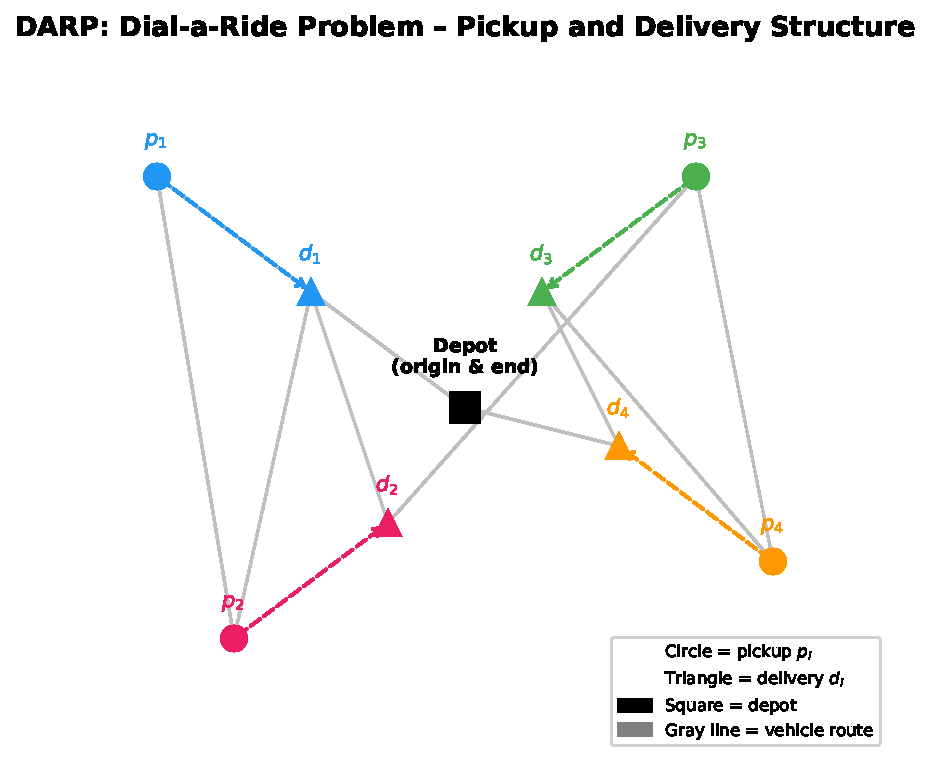
\includegraphics[width=0.75\linewidth]{darp_overview.pdf}
    \caption{DARP structure: the depot (square), pickup nodes (circles), and
    delivery nodes (triangles).  Dashed arrows show each request's travel
    direction; the gray line shows one possible vehicle route.}
  \end{figure}

  \framebreak

  \textbf{Static vs.\ Dynamic DARP.}  In the \emph{static} variant, all
  requests are known before routes are planned (e.g., pre-booked the day
  before).  In the \emph{dynamic} variant, requests arrive in real time during
  service and must be inserted into existing routes with minimal disruption.
  The dynamic version requires fast re-optimisation and is especially relevant
  for urban dial-a-ride operations.

  \begin{alertblock}{Key Insight}
    The combination of pickup-before-delivery precedence constraints with a
    \emph{bounded ride time} is what makes DARP fundamentally harder than
    standard VRPTW.  The constraint that customer $i$ must be onboard at most
    $L_i$ time units means that feasibility checking itself requires careful
    scheduling, and many neighbourhood moves that are feasible in VRPTW become
    infeasible in DARP.
  \end{alertblock}

\end{frame}

%% ============================================================
\section{Problem Formulation}
%% ============================================================

\begin{frame}[allowframebreaks]{Mathematical Formulation of DARP}

  We follow the formulation presented by Cordeau and Laporte (2003) and
  Parragh, Doerner, and Hartl (2008).  The model is the most widely used
  basis for both exact and heuristic approaches.

  \textbf{Sets and notation.}  Let $n$ be the number of transportation
  requests, numbered $1, \ldots, n$.  Each request $i$ has:
  \begin{itemize}
    \item a \textbf{pickup node} $i \in P = \{1,\ldots,n\}$, and
    \item a \textbf{delivery node} $n+i \in D = \{n+1,\ldots,2n\}$.
  \end{itemize}
  The depot is represented by two copies: node $0$ (vehicle start) and node
  $2n+1$ (vehicle end).  The complete node set is
  $V = \{0\} \cup P \cup D \cup \{2n+1\}$.

  We have a homogeneous fleet of $m$ vehicles, each with capacity $Q$.  The
  travel time between nodes $i$ and $j$ is $t_{ij}$; the service time at node
  $i$ is $s_i$; and node $i$ has a \textbf{time window} $[e_i, l_i]$ meaning
  service must start no earlier than $e_i$ and no later than $l_i$.  The
  maximum ride time for request $i$ is $L_i$, and the maximum route duration
  is $T$.

  \framebreak

  \textbf{Decision variables.}
  \begin{itemize}
    \item $x_{ijk} \in \{0,1\}$: equals 1 if vehicle $k$ travels directly
          from node $i$ to node $j$.
    \item $B_{ik}$: the time at which vehicle $k$ begins service at node $i$.
    \item $Q_{ik}$: the load of vehicle $k$ when it \emph{leaves} node $i$.
    \item $L_{ik}$: the ride time of customer $i$ on vehicle $k$.
  \end{itemize}

  \framebreak

  \begin{block}{DARP: The Whole Problem (7.3.1)}
    \textbf{Objective — minimise total route duration:}
    \[
      \min \; \sum_{k=1}^{m} \sum_{i \in V} \sum_{j \in V} c_{ij}\, x_{ijk}
    \]
    where $c_{ij}$ is the cost (typically travel time or distance) of arc
    $(i,j)$.  The sum counts every arc traversed by any vehicle.

    \medskip
    \textbf{Constraints:}
    \begin{align}
      \sum_{k=1}^{m} \sum_{j \in V} x_{ijk} &= 1
        & \forall i \in P \tag{C1} \\
      \sum_{j \in V} x_{0jk} &= 1
        & \forall k \tag{C2} \\
      \sum_{i \in V} x_{ihk} - \sum_{j \in V} x_{hjk} &= 0
        & \forall h \in P \cup D,\; \forall k \tag{C3} \\
      \sum_{i \in V} x_{i,2n+1,k} &= 1
        & \forall k \tag{C4}
    \end{align}
  \end{block}

  \framebreak

  \begin{block}{Capacity, Time, and Ride-Time Constraints}
    \begin{align}
      Q_{ik} &= Q_{jk} + q_j \quad\text{if } x_{ijk}=1
        & \forall i,j,k \tag{C5} \\
      0 \leq Q_{ik} &\leq Q
        & \forall i,k \tag{C6} \\
      B_{jk} &\geq B_{ik} + s_i + t_{ij} \quad\text{if } x_{ijk}=1
        & \forall i,j,k \tag{C7} \\
      e_i \leq B_{ik} &\leq l_i
        & \forall i,k \tag{C8} \\
      L_{ik} &= B_{n+i,k} - (B_{ik} + s_i)
        & \forall i \in P, \; \forall k \tag{C9} \\
      t_{i,n+i} \leq L_{ik} &\leq L_i
        & \forall i \in P, \; \forall k \tag{C10} \\
      B_{2n+1,k} - B_{0k} &\leq T
        & \forall k \tag{C11}
    \end{align}
  \end{block}

  \framebreak

  \textbf{Interpretation of each constraint group:}

  \begin{itemize}
    \item \textbf{(C1)}: Every request is served by exactly one vehicle.
          This ensures no customer is left unserved or served twice.
    \item \textbf{(C2)--(C4)}: Flow balance.  Each vehicle leaves the depot
          once (C2), has equal inflow and outflow at every intermediate node
          (C3), and returns to the depot once (C4).
    \item \textbf{(C5)--(C6)}: Capacity tracking.  The load $Q_{ik}$
          increases by $q_j$ (request load) after picking up customer $j$
          and decreases after delivery.  At no point may the load exceed $Q$.
    \item \textbf{(C7)--(C8)}: Time propagation and time windows.  Service at
          $j$ cannot start before completing service at $i$ plus travel
          $t_{ij}$, and all service times must fall within time windows
          $[e_i, l_i]$.
    \item \textbf{(C9)--(C10)}: Ride time.  The ride time $L_{ik}$ of
          customer $i$ on vehicle $k$ equals the gap between starting delivery
          service and finishing pickup service.  It must be at least the direct
          travel time $t_{i,n+i}$ and at most the maximum $L_i$.
    \item \textbf{(C11)}: Route duration bound $T$.
  \end{itemize}

  \framebreak

  \begin{figure}[ht]
    \centering
    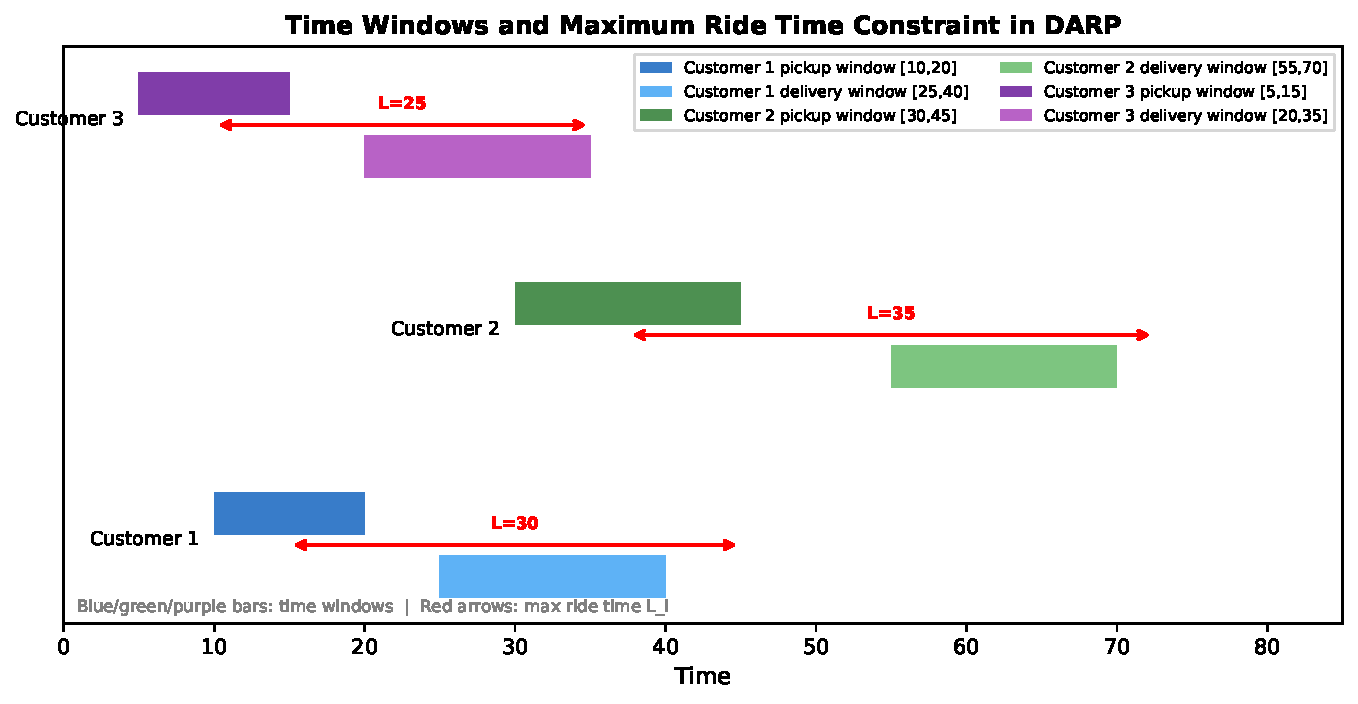
\includegraphics[width=0.85\linewidth]{time_windows_darp.pdf}
    \caption{Time windows (coloured bars) at pickup and delivery nodes for
    three customers.  The red double-headed arrows indicate the maximum ride
    time $L_i$ for each customer.  The delivery window must be consistent with
    finishing the pickup and the direct ride.}
  \end{figure}

  \framebreak

  \begin{figure}[ht]
    \centering
    
\includegraphics[width=0.80\linewidth]{darp_constraints.pdf}
    \caption{Visual taxonomy of the five main DARP constraint types.  Each box
    summarises the constraint category, the mathematical symbol(s) involved,
    and its practical meaning.}
  \end{figure}

  \framebreak

  \textbf{LP relaxation and integer programming.}  The DARP (7.3.1) as
  stated is a Mixed-Integer Program (MIP).  Its LP relaxation — obtained by
  dropping the integrality requirements on $x_{ijk}$ — is solved at each
  node of the branch-and-bound tree in exact methods.  When the vehicle
  capacity $Q \geq 1$ is a continuous fraction, equations (C5) reduce to
  a simpler LP network-flow structure; the difficulty arises because the
  $x_{ijk}$ variables are binary.

  One important observation: if the fractional $x_{ijk}^*$ satisfies
  $x_{ijk}^* < 1$ for all arcs, then the optimal LP value provides a lower
  bound that exact algorithms use to prune the search tree.  Strengthening
  this bound via \emph{cutting planes} is the core idea of branch-and-cut,
  as discussed next.

\end{frame}

%% ============================================================
\section{Solution Methods for DARP}
%% ============================================================

\begin{frame}[allowframebreaks]{Exact Methods: Branch-and-Cut (Cordeau 2006)}

  The DARP is NP-hard.  Exact methods guarantee an optimal solution but are
  computationally feasible only for moderate-sized instances (up to roughly
  $n \approx 8$ requests per vehicle, $m \leq 3$ vehicles in reasonable time).
  The state-of-the-art exact approach is the \textbf{branch-and-cut} algorithm
  of Cordeau (2006), which combines:
  \begin{enumerate}
    \item Linear programming (LP) relaxation at each tree node.
    \item Valid inequalities (\emph{cutting planes}) to tighten the LP bound.
    \item Branching on fractional arc variables.
  \end{enumerate}

  \begin{block}{Branch-and-Cut Framework}
    \begin{enumerate}
      \item Solve LP relaxation of the DARP formulation.
      \item If the LP solution is integer-feasible: update incumbent if better,
            backtrack.
      \item Else, separate violated valid inequalities.  If found, add them and
            go to step 1.  Otherwise, branch on a fractional variable
            $x_{ijk}^* \in (0,1)$, creating two child nodes.
      \item Prune a node if its LP lower bound exceeds the current incumbent.
    \end{enumerate}
  \end{block}

  \framebreak

  \begin{figure}[ht]
    \centering
    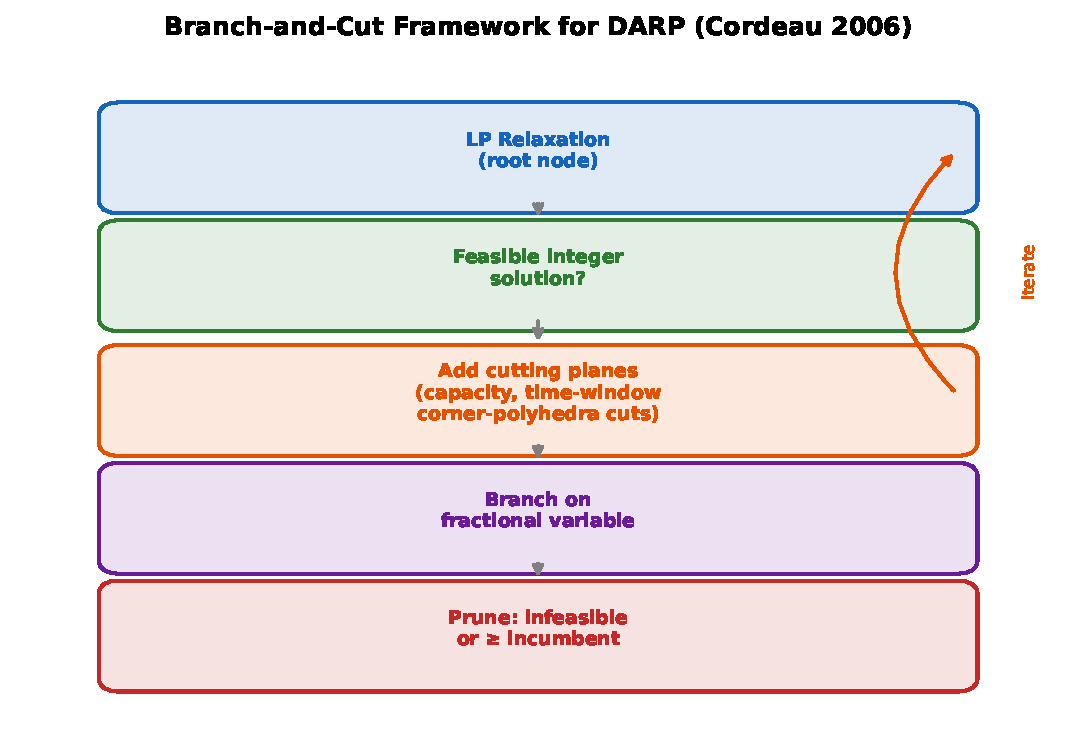
\includegraphics[width=0.50\linewidth]{branch_cut_framework.pdf}
    \caption{Schematic of the branch-and-cut framework for DARP.  The iterate
    arrow (right side) shows that cutting planes can be added in multiple rounds
    before a branching decision is made, tightening the LP relaxation.}
  \end{figure}

  \framebreak

  \textbf{Key classes of valid inequalities used in DARP branch-and-cut:}

  \begin{itemize}
    \item \textbf{Capacity cuts}: ensure that any subset $S$ of requests
          cannot be served with fewer vehicles than required by their combined
          load.  These are analogous to capacity cuts in CVRP branch-and-cut.
    \item \textbf{Time-window strengthening}: propagating the time-window
          tightness through the sequence of visits eliminates fractional
          solutions that would violate temporal feasibility.
    \item \textbf{Corner-polyhedra cuts}: when a scheduling subproblem has a
          fractional solution, cutting planes from the corner polyhedron of
          the scheduling polytope can be added to strengthen the formulation.
    \item \textbf{Precedence cuts}: the requirement that $p_i$ precedes
          $d_i$ on the same route generates logical implications on arc
          variables that can be turned into linear inequalities.
  \end{itemize}

  Cordeau (2006) showed that on the standard benchmark instances (up to
  $n = 6$ requests and $m = 3$ vehicles), the branch-and-cut finds provably
  optimal solutions within reasonable CPU time.  Larger instances require
  heuristic methods.

  \begin{alertblock}{Key Insight}
    The principal bottleneck for exact DARP methods is the interaction between
    capacity and scheduling constraints: every branching decision that fixes a
    route arc immediately propagates time and load information, creating a
    highly constrained sub-MIP.  Cutting planes that tighten both the
    capacity and the scheduling polytopes simultaneously are therefore the
    most valuable.
  \end{alertblock}

\end{frame}

\begin{frame}[allowframebreaks]{Heuristic Methods: Insertion and Improvement}

  Because exact methods are limited to small instances, practitioners rely on
  \textbf{heuristic} approaches that trade optimality guarantees for speed.
  Two classical families are relevant:

  \textbf{1. Insertion heuristics.}  These build routes from scratch by
  iteratively selecting the ``cheapest feasible'' insertion position for each
  unrouted request.  The algorithm terminates when all requests have been
  inserted or it is declared infeasible to do so (requiring a new vehicle).

  \begin{block}{Generic Insertion Heuristic for DARP}
    \begin{enumerate}
      \item Initialise: routes $R_1, \ldots, R_m$ each containing only the
            depot.
      \item Select unrouted request $i$ (e.g., earliest time window first).
      \item For each route $R_k$ and each pair of positions $(\pi_p, \pi_d)$
            (where $\pi_p < \pi_d$) in $R_k$: compute the \emph{insertion
            cost} $\Delta c(i, \pi_p, \pi_d, R_k)$ = increase in route cost
            from inserting $p_i$ at position $\pi_p$ and $d_i$ at $\pi_d$.
      \item Check feasibility: time windows, capacity, ride time $L_i$ all
            satisfied after insertion.
      \item Insert request $i$ into the cheapest feasible slot found.  If
            none exists, open a new vehicle route.
      \item Repeat from step 2 until all requests are assigned.
    \end{enumerate}
  \end{block}

  \framebreak

  \begin{figure}[ht]
    \centering
    
\includegraphics[width=0.90\linewidth]{insertion_heuristic.pdf}
    \caption{Three successive steps of a DARP insertion heuristic.  At each
    step, the next request (red crosses) is inserted at the cheapest feasible
    position in the growing route (green).  The route gradually grows as more
    requests are accommodated.}
  \end{figure}

  \framebreak

  \begin{exampleblock}{Worked Example: Insertion Cost Calculation}
    Suppose the current route visits nodes $[D, p_1, d_1, D]$ in order, with
    travel times $t_{D,p_1}=5$, $t_{p_1,d_1}=3$, $t_{d_1,D}=4$.
    The current cost is $5+3+4=12$.

    Now we want to insert request 2 with pickup $p_2$ and delivery $d_2$.
    Consider inserting $p_2$ between $p_1$ and $d_1$, and $d_2$ between
    $d_1$ and $D$.  The new route is $[D, p_1, p_2, d_1, d_2, D]$.
    New cost: $t_{D,p_1}+t_{p_1,p_2}+t_{p_2,d_1}+t_{d_1,d_2}+t_{d_2,D}$.
    If $t_{p_1,p_2}=2$, $t_{p_2,d_1}=4$, $t_{d_1,d_2}=3$, $t_{d_2,D}=5$,
    new cost $= 5+2+4+3+5=19$.  Insertion cost $= 19-12=7$.

    Before accepting, we check: (a) capacity does not exceed $Q$ at any
    position; (b) time windows $[e_{p_2}, l_{p_2}]$ and $[e_{d_2}, l_{d_2}]$
    are satisfied; (c) ride time $B_{d_2,k} - (B_{p_2,k} + s_{p_2}) \leq L_2$.
    Only if all three checks pass is this insertion accepted.
  \end{exampleblock}

  \framebreak

  \textbf{2. Improvement heuristics: 2-opt and 3-opt for DARP.}  After
  obtaining an initial solution, local search operators attempt to reduce
  cost by reconfiguring parts of the routes.  The classical \emph{2-opt}
  move for TSP reverses a segment of a route.  For DARP, this operator must
  be modified to preserve:
  \begin{itemize}
    \item Pickup-before-delivery precedence for every request affected.
    \item Time-window feasibility at every node.
    \item Maximum ride-time feasibility for every passenger.
  \end{itemize}
  This makes feasibility checking more expensive than in TSP; efficient data
  structures that propagate the earliest and latest feasible service times
  (``forward time slack'' and ``backward time slack'') allow checking in
  $O(1)$ per move after $O(n)$ preprocessing.

  \begin{alertblock}{Key Insight}
    The high density of DARP constraints means that the feasible neighbourhood
    is much smaller than in VRPTW.  Consequently, heuristics that can escape
    infeasibility — such as allowing temporary constraint violations with a
    penalty — tend to outperform strictly feasibility-preserving methods.
  \end{alertblock}

\end{frame}

\begin{frame}[allowframebreaks]{Metaheuristics for DARP}

  Metaheuristics are higher-level strategies that guide local search to
  escape local optima.  Three families dominate the DARP literature.

  \medskip
  \textbf{Tabu Search (TS).}  The idea behind tabu search is to allow moves
  to temporarily \emph{worse} solutions, preventing cycling by declaring
  recently visited solutions or recently used moves \emph{tabu} (forbidden)
  for a number of iterations.  For DARP, Cordeau and Laporte (2003) developed
  an influential TS algorithm where the ``move'' is a \emph{request relocation}:
  a single request $i$ is removed from its current route and re-inserted into
  the same or another route at the cheapest feasible position.

  \begin{block}{Tabu Search for DARP (Cordeau \& Laporte 2003)}
    \begin{enumerate}
      \item Generate initial solution $s$ (e.g., via insertion heuristic).
      \item Repeat until stopping criterion (iteration limit or time limit):
        \begin{enumerate}
          \item[2a.] For each request $i$ and each candidate insertion
                     position $(\pi_p, \pi_d)$ on all routes: compute move
                     cost $\delta(i, \pi_p, \pi_d)$.
          \item[2b.] Determine the best non-tabu move (or a tabu move if it
                     yields a new best solution — \emph{aspiration criterion}).
          \item[2c.] Execute the move; update tabu list (mark the reverse
                     move tabu for $\theta$ iterations).
          \item[2d.] If current solution is better than best known, update
                     incumbent $s^*$.
        \end{enumerate}
      \item Return $s^*$.
    \end{enumerate}
  \end{block}

  \framebreak

  \begin{figure}[ht]
    \centering
    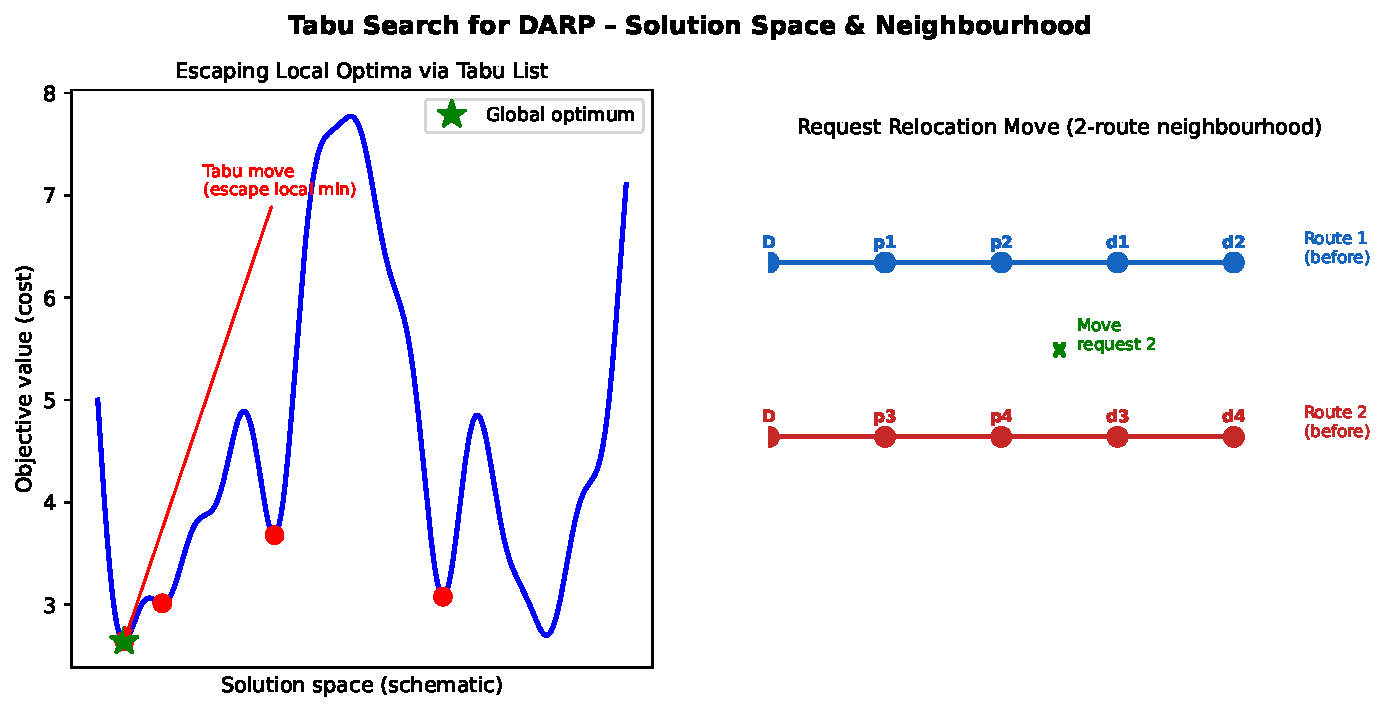
\includegraphics[width=0.80\linewidth]{tabu_search_darp.pdf}
    \caption{Left: schematic objective landscape for DARP.  Tabu search
    allows uphill moves (red circles = local optima) to reach the global
    optimum (green star).  Right: a ``request relocation'' neighbourhood
    move — request 2 is moved from Route 1 to Route 2.}
  \end{figure}

  \framebreak

  \textbf{An important implementation detail for DARP tabu search: penalty
  functions.}  Cordeau and Laporte (2003) allow constraint violations during
  the search, penalising excess ride time, excess load, and violated time
  windows in the objective:
  \[
    f(s) = \text{cost}(s)
           + \alpha \cdot \text{ExcessRideTime}(s)
           + \beta  \cdot \text{ExcessLoad}(s)
           + \gamma \cdot \text{TimeWindowViolation}(s)
  \]
  The penalty parameters $\alpha, \beta, \gamma > 0$ are adjusted
  \emph{dynamically} during the search: if the current solution is feasible,
  they increase to push the search back towards feasibility; if infeasible,
  they decrease to allow more exploration.  This self-regulating mechanism
  has been shown to be highly effective in practice.

  \framebreak

  \textbf{Large Neighbourhood Search (LNS) / Adaptive LNS (ALNS).}
  The idea of LNS, due to Shaw (1998), is to \emph{destroy} a large portion
  of the current solution (removing $q$ requests from their routes) and then
  \emph{repair} it (re-inserting the removed requests in the cheapest feasible
  way).  Because $q$ can be large (e.g., $q = 5$--$30$), LNS explores a
  much larger neighbourhood than single-request relocation moves.

  \begin{figure}[ht]
    \centering
    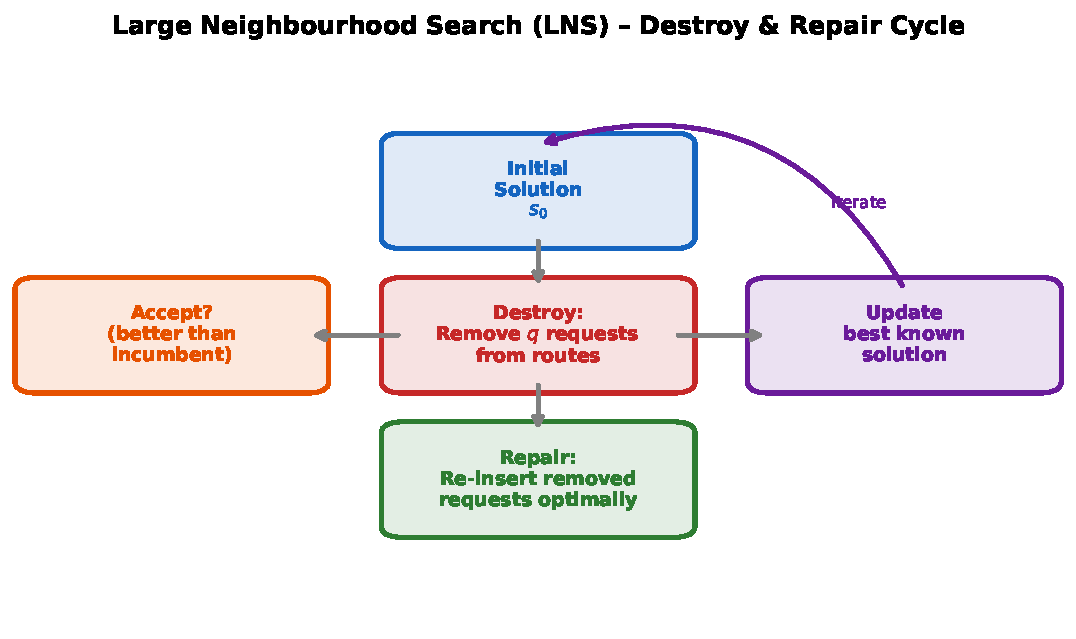
\includegraphics[width=0.55\linewidth]{lns_cycle.pdf}
    \caption{The Destroy-Repair cycle of Large Neighbourhood Search.  After
    repair, the new solution is accepted if it improves the incumbent; the
    best solution is tracked throughout and returned at termination.}
  \end{figure}

  \framebreak

  Ropke and Pisinger (2006) extended LNS to \textbf{Adaptive LNS (ALNS)} by
  maintaining multiple destroy and repair operators and adaptively selecting
  them based on their historical performance.  The operator selection follows
  a roulette-wheel mechanism: each operator's weight is updated after each
  iteration based on whether it contributed to a new best solution.  For DARP,
  the destroy operators include:
  \begin{itemize}
    \item \textbf{Random removal}: select $q$ requests uniformly at random.
    \item \textbf{Worst removal}: remove the $q$ requests contributing most
          to the objective (most expensive rides).
    \item \textbf{Related removal} (Shaw 1998): remove $q$ requests that are
          \emph{similar} in time, location, or load — intuition is that
          similar requests can ``swap'' routes effectively.
    \item \textbf{Shaw removal with ride-time focus}: remove requests with the
          longest actual ride time first, as these are most likely causing
          constraint violations.
  \end{itemize}

  \framebreak

  \begin{exampleblock}{Worked Example: Related Removal}
    Consider 5 requests with the following direct travel time from a
    reference request $r$:
    $t(r,1)=2$, $t(r,2)=8$, $t(r,3)=3$, $t(r,4)=1$, $t(r,5)=6$.
    Their time-window similarity scores (smaller = more similar):
    $\sigma_1=4$, $\sigma_2=1$, $\sigma_3=5$, $\sigma_4=2$, $\sigma_5=3$.

    A relatedness measure combining distance and time:
    $\rho(r,i) = \lambda \cdot t(r,i) + (1-\lambda) \cdot \sigma_i$, with
    $\lambda=0.5$:
    $\rho(r,1)=3$, $\rho(r,2)=4.5$, $\rho(r,3)=4$, $\rho(r,4)=1.5$,
    $\rho(r,5)=4.5$.

    Sorting by $\rho$: requests $4, 1, 3, 2, 5$.
    If $q=3$, we remove requests $\{r, 4, 1\}$ — the three most related ones
    — and re-insert them using a greedy insertion repair.
  \end{exampleblock}

  \framebreak

  \textbf{Population-based methods and hybrid approaches.}  Beyond single-
  solution metaheuristics, the literature includes:
  \begin{itemize}
    \item \textbf{Genetic algorithms}: encode DARP routes as chromosomes
          and apply crossover and mutation operators.  The challenge is that
          standard GA crossover (e.g., order-crossover) can violate
          pickup-before-delivery precedence, so specialised crossover operators
          are needed.
    \item \textbf{Simulated annealing}: the ``annealing'' analogy comes from
          controlled cooling of metals — a slow temperature decrease makes
          the search accept worse solutions with decreasing probability,
          allowing global exploration early and exploitation later.
    \item \textbf{Branch-and-price with heuristic pricing}: in column-
          generation approaches, each feasible DARP route (column) is
          generated by solving a resource-constrained shortest-path problem.
          Heuristic pricing replaces exact labelling when the latter is too
          slow.
  \end{itemize}

  \begin{alertblock}{Key Insight}
    Across the DARP literature, metaheuristics — particularly tabu search
    and LNS/ALNS — consistently outperform pure constructive heuristics
    by 1--5\% in solution quality, and they scale to hundreds of requests
    while exact methods stall at tens.  The penalty-based infeasibility
    tolerance is the single most impactful design choice for tabu search.
  \end{alertblock}

\end{frame}

\begin{frame}[allowframebreaks]{Benchmark Instances and Computational Results}

  The standard benchmark for DARP research is the set of instances introduced
  by Cordeau and Laporte (2003), denoted \texttt{a} (easy) and \texttt{b}
  (harder), with varying numbers of requests ($n = 24, 36, 48, 72, 96$) and
  vehicle fleet sizes ($m = 2, 3, \ldots, 13$).  Each instance specifies
  a maximum route duration $T$, maximum ride time $L$, and vehicle capacity $Q$.

  \begin{figure}[ht]
    \centering
    
\includegraphics[width=0.85\linewidth]{benchmark_comparison.pdf}
    \caption{Schematic comparison of DARP solution methods on standard
    benchmark instances.  Left: average gap from best known solution (lower
    is better).  Right: typical CPU time (log scale).  Branch-and-Cut
    achieves the best quality but requires orders of magnitude more time than
    metaheuristics for large instances.}
  \end{figure}

  \framebreak

  \textbf{Observations from benchmark results:}
  \begin{itemize}
    \item Branch-and-cut (Cordeau 2006) solves instances up to $n \approx 8$
          requests per vehicle optimally; beyond this, computing time becomes
          prohibitive.
    \item The tabu search of Cordeau and Laporte (2003) finds solutions within
          1\% of optimum on small instances and remains the reference for
          medium instances ($n \leq 96$).
    \item ALNS (Ropke and Pisinger 2006) achieves the best solution quality on
          large instances and runs faster per iteration than tabu search due
          to simpler neighbourhood evaluation.
    \item Dynamic programming heuristics (Lim et al.\ 2010) handle
          single-vehicle instances optimally but do not scale to multi-vehicle
          problems.
  \end{itemize}

  \begin{exampleblock}{Worked Example: Reading a Cordeau-Laporte Instance}
    Instance \texttt{a2-16} has $n=16$ requests, $m=2$ vehicles, $Q=6$
    passengers, $T=480$ minutes, $L=90$ minutes.  The 16 requests are
    distributed in a $[-10,10]^2$ Euclidean plane.  A solver would seek
    two routes each visiting at most 16 pickup/delivery pairs, each
    respecting time windows on each node, each with route duration $\leq 480$,
    and each passenger's ride time $\leq 90$.
  \end{exampleblock}

\end{frame}

%% ── Python code frame ────────────────────────────────────────────────────────
\begin{frame}[fragile]{Python Implementation: DARP Insertion Heuristic}
\begin{lstlisting}[caption={DARP insertion heuristic skeleton (Python 3)},
                   label=lst:darp_insertion]
import numpy as np
from itertools import permutations

def darp_insertion_heuristic(requests, n_vehicles, capacity, max_ride_time, travel_time):
    """
    Simple DARP insertion heuristic.
    requests: list of dict with keys: pickup, delivery, load, e_p, l_p, e_d, l_d
    travel_time: 2D numpy array, travel_time[i][j] = time from i to j
    Returns: list of routes (each route = ordered list of node indices)
    """
    DEPOT_START, DEPOT_END = 0, 2*len(requests) + 1
    routes = [[DEPOT_START, DEPOT_END] for _ in range(n_vehicles)]
    service_times = [0.0] * (2*len(requests) + 2)  # B[i] for each node

    def check_feasibility(route, svc):
        """Check time window + ride time + capacity along a route."""
        load, t = 0, 0.0
        for idx, node in enumerate(route):
            if idx > 0:
                t = max(t + travel_time[route[idx-1], node], 0)
            if node == DEPOT_START or node == DEPOT_END:
                continue
            req_idx = (node - 1) % len(requests)
            req = requests[req_idx]
            is_pickup = (node - 1) < len(requests)
            ew = req['e_p'] if is_pickup else req['e_d']
            lw = req['l_p'] if is_pickup else req['l_d']
            if t > lw:
                return False
            t = max(t, ew)
            svc[node] = t
            load += req['load'] if is_pickup else -req['load']
            if not (0 <= load <= capacity):
                return False
        for i, req in enumerate(requests):
            pickup_node, delivery_node = i + 1, len(requests) + i + 1
            if pickup_node in route and delivery_node in route:
                ride = svc[delivery_node] - svc[pickup_node]
                if ride > max_ride_time:
                    return False
        return True

    unrouted = list(range(len(requests)))
    for req_idx in unrouted:
        pickup = req_idx + 1
        delivery = len(requests) + req_idx + 1
        best_cost, best_route_idx, best_pos = float('inf'), -1, None
        for k, route in enumerate(routes):
            for i in range(1, len(route)):         # pickup position
                for j in range(i, len(route)):     # delivery position >= pickup
                    new_route = route[:i] + [pickup] + route[i:j] + [delivery] + route[j:]
                    svc = service_times[:]
                    if check_feasibility(new_route, svc):
                        cost = sum(travel_time[new_route[m], new_route[m+1]]
                                   for m in range(len(new_route)-1))
                        if cost < best_cost:
                            best_cost, best_route_idx, best_pos = cost, k, (i, j, new_route)
        if best_pos is not None:
            routes[best_route_idx] = best_pos[2]
        # else: infeasible insertion -> open new vehicle (not shown)
    return routes
\end{lstlisting}
\end{frame}

%% ============================================================
\section{Other Pickup and Delivery of People Problems}
%% ============================================================

\begin{frame}[allowframebreaks]{School Bus Routing Problem (SBRP)}

  The \textbf{School Bus Routing Problem (SBRP)} is one of the most
  practically important PDP-People variants.  It differs from DARP in
  several structural ways:

  \begin{block}{SBRP vs.\ DARP: Key Structural Differences}
    \begin{tabular}{p{0.45\linewidth} p{0.45\linewidth}}
      \toprule
      \textbf{DARP} & \textbf{SBRP} \\
      \midrule
      Door-to-door service & Pickup at designated \emph{bus stops} \\
      One depot            & One or more \emph{schools} as destinations \\
      Heterogeneous time   & Fixed bell times (hard deadlines) \\
      Max ride time $L_i$  & Walk distance $\leq W_{\max}$ from home to stop \\
      General fleet        & School buses (homogeneous or heterogeneous) \\
      \bottomrule
    \end{tabular}
  \end{block}

  \framebreak

  The SBRP consists of two interrelated subproblems:
  \begin{enumerate}
    \item \textbf{Bus stop selection}: choose which candidate stops to
          activate, ensuring every student lives within $W_{\max}$ walking
          distance of at least one active stop.
    \item \textbf{Route generation and assignment}: design bus routes that
          visit the selected stops, pick up students, and arrive at the school
          on time.
  \end{enumerate}
  These two subproblems are often solved sequentially (first stop selection,
  then routing), but joint optimisation yields better solutions.

  \begin{figure}[ht]
    \centering
    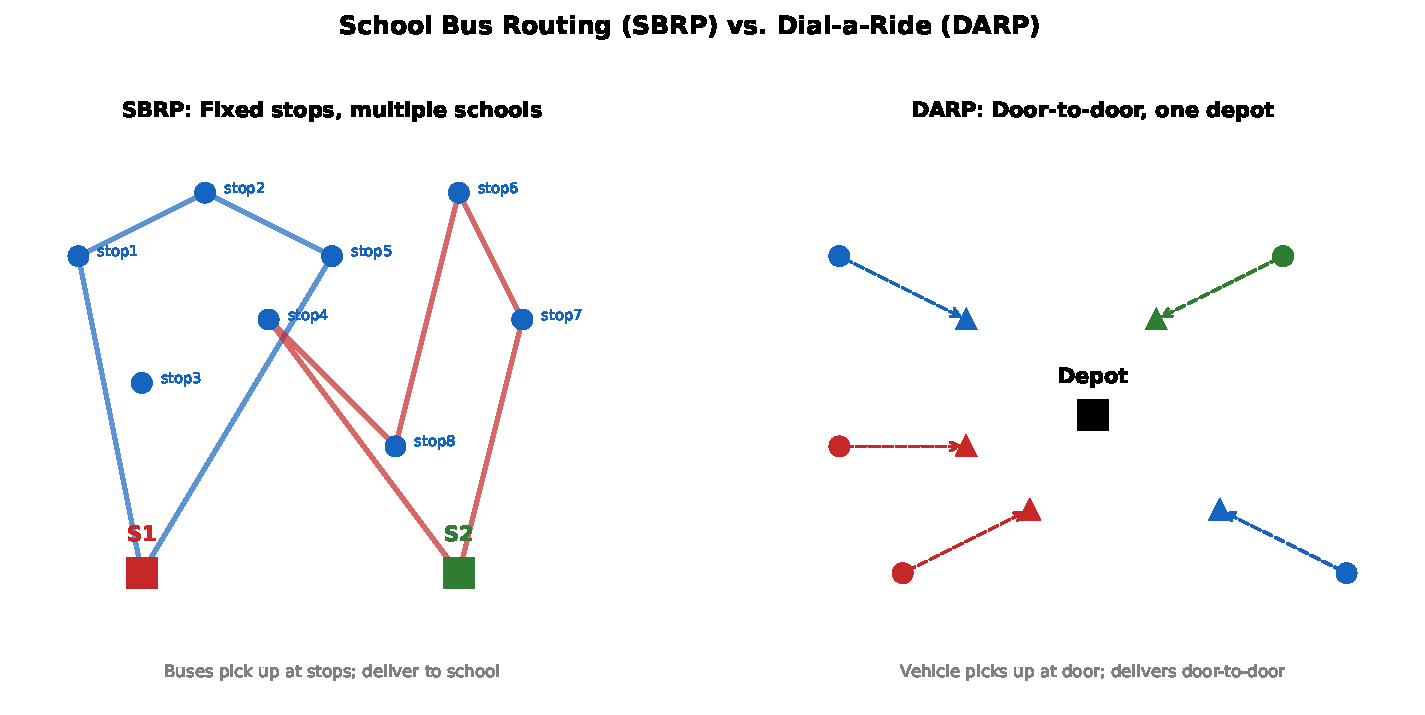
\includegraphics[width=0.75\linewidth]{sbrp_vs_darp.pdf}
    \caption{Left: SBRP with fixed stops (circles) and two schools (squares).
    Buses collect students from stops and deliver to schools on two separate
    routes.  Right: DARP with door-to-door service from a single depot.}
  \end{figure}

  \framebreak

  \textbf{Solution approaches for SBRP.}  Park and Kim (2010) provide a
  thorough survey.  The most successful methods include:
  \begin{itemize}
    \item \textbf{GIS-based clustering}: students are first grouped into
          clusters by geographic proximity; each cluster is served by one bus.
          A Branch-and-Cut algorithm then optimises the routing within each
          cluster.
    \item \textbf{Mixed-integer programming}: for small instances, the joint
          stop-selection and routing problem can be solved exactly using CPLEX
          or Gurobi with the formulation of Bowman and Casto (1981).
    \item \textbf{Metaheuristics}: genetic algorithms (with cluster-first/
          route-second encoding), tabu search, and simulated annealing are all
          applied in the literature; differences of 5--20\% in fleet size are
          reported between methods.
  \end{itemize}

  \begin{alertblock}{Key Insight}
    SBRP has a \emph{spatial pre-processing} step — stop selection — that has
    no analogue in DARP.  The walk-distance constraint couples the stop
    selection to the demographic distribution of students, making it a
    bi-level problem in general.
  \end{alertblock}

\end{frame}

\begin{frame}[allowframebreaks]{Demand Responsive Transit (DRT)}

  \textbf{Demand Responsive Transit (DRT)} occupies a middle ground between
  fixed-line public transport (rigid timetables and fixed routes) and pure
  dial-a-ride (fully flexible door-to-door).  DRT services operate on
  partially flexible routes that can deviate from a baseline path to serve
  on-demand pickup and delivery requests.

  \begin{figure}[ht]
    \centering
    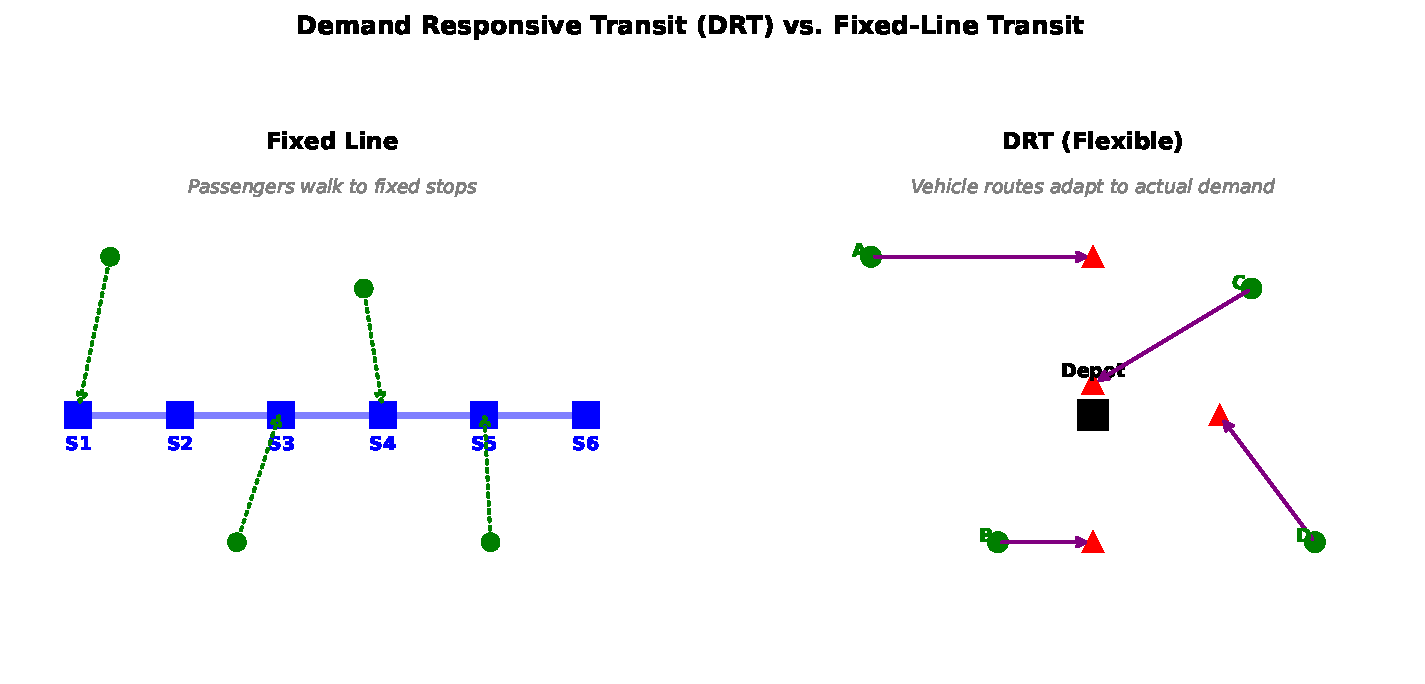
\includegraphics[width=0.80\linewidth]{drt_concept.pdf}
    \caption{Left: fixed-line transit — passengers walk to fixed stops (S1--S6)
    along a predetermined route.  Right: DRT — the vehicle route adapts
    to the actual distribution of demand, picking up passengers closer to
    their origins and delivering them nearer their destinations.}
  \end{figure}

  \framebreak

  \textbf{The ``deviation'' model for DRT.}  In the deviation model, each
  vehicle follows a \emph{backbone route} that connects major activity centres.
  It is allowed to deviate by at most $\Delta$ minutes from this backbone to
  serve on-demand passengers.  This constraint limits the service area and
  simplifies scheduling, at the cost of some flexibility.

  \begin{block}{DRT Deviation Constraint}
    Let $\tau_{\text{backbone}}(v)$ be the scheduled arrival time of vehicle
    $v$ at backbone node $b_j$, and $\tau_{\text{actual}}(v)$ the actual
    arrival.  The constraint is:
    \[
      |\tau_{\text{actual}}(v, b_j) - \tau_{\text{backbone}}(v, b_j)| \leq \Delta
      \quad \forall j,\, \forall v
    \]
    This ensures that connecting passengers relying on backbone timetables
    are not disappointed by large deviations.
  \end{block}

  \framebreak

  \textbf{Online vs.\ offline DRT planning.}  When requests are known in
  advance (\emph{offline}), DRT reduces to a DARP with additional
  backbone-deviation constraints, solvable by standard DARP metaheuristics.
  When requests arrive in real time (\emph{online}), the system must re-route
  vehicles while in service, using:
  \begin{itemize}
    \item \textbf{Rolling horizon}: periodically re-solve the DARP for the
          next time horizon of $H$ minutes using current vehicle positions as
          new depot locations.
    \item \textbf{Event-driven insertion}: each new request triggers a fast
          insertion into the current schedule; if infeasible, the request is
          rejected or deferred.
  \end{itemize}

  \begin{alertblock}{Key Insight}
    The key distinction of DRT from pure DARP is that DRT must respect a
    backbone timetable, limiting route deviations.  This additional constraint
    can actually simplify the scheduling problem in some cases (fewer possible
    insertion positions) while adding complexity in others (backbone
    synchronisation requirements).
  \end{alertblock}

\end{frame}

\begin{frame}[allowframebreaks]{Car Pooling and Ride Sharing}

  \textbf{Car pooling} (or \emph{carpooling}) refers to the problem of
  assigning passengers with overlapping origin–destination paths to shared
  vehicles, reducing the total number of vehicle trips.  Unlike DARP, the
  vehicles in car pooling are typically private cars whose owners
  (\emph{drivers}) are also passengers with their own origin and destination.

  \begin{figure}[ht]
    \centering
    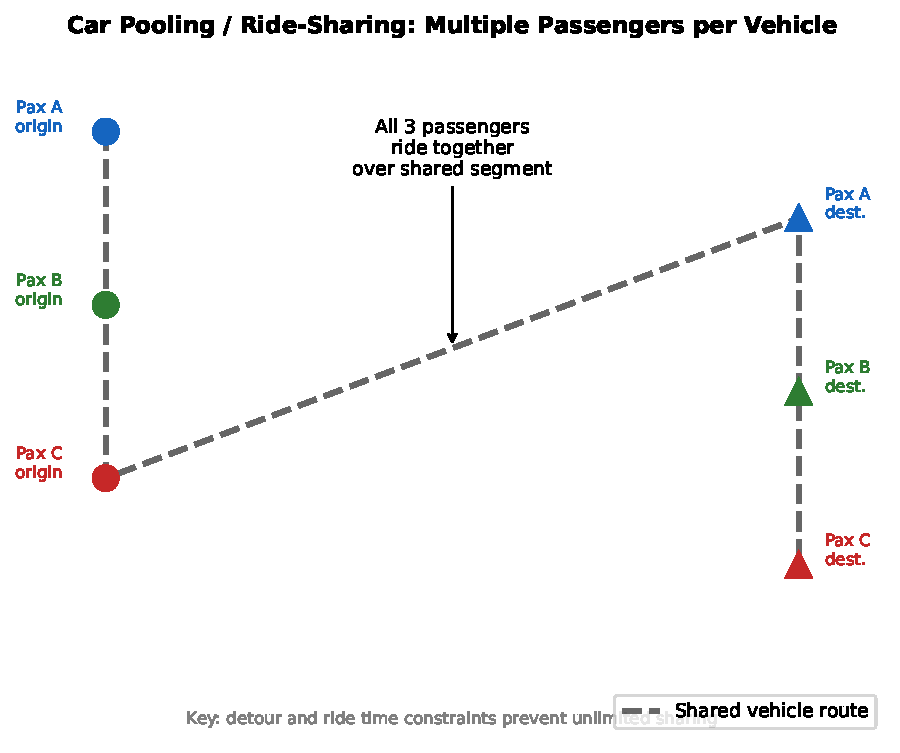
\includegraphics[width=0.60\linewidth]{carpooling_network.pdf}
    \caption{Three passengers (A, B, C) with different origins (circles) and
    destinations (triangles) sharing one vehicle.  The vehicle picks up all
    three near the common starting area and drops them off near their
    respective destinations, following the shared segment in the middle.}
  \end{figure}

  \framebreak

  \textbf{The car pooling problem formulation.}  The car pooling problem
  can be modelled as a variant of DARP where:
  \begin{itemize}
    \item Each driver $d$ is both a \emph{vehicle provider} (contributing
          capacity $q_d$) and a \emph{passenger} with their own request
          $(o_d, \delta_d)$.
    \item A passenger $p$ is assigned to driver $d$ only if the detour
          incurred by $d$ to pick up and drop off $p$ does not exceed
          $\Delta_d$ (driver's acceptable detour).
    \item The objective minimises total vehicle-kilometres driven (or
          equivalently maximises sharing, reducing total trips).
  \end{itemize}

  \begin{block}{Detour Constraint for Car Pooling}
    Let $\text{dist}(o_d, \delta_d)$ be the direct distance for driver $d$.
    If driver $d$ picks up passenger $p$ at $o_p$ and drops off at $\delta_p$,
    the detour is:
    \[
      \text{detour}(d, p) = \text{dist}(o_d, o_p) + \text{dist}(o_p, \delta_p)
                           + \text{dist}(\delta_p, \delta_d) - \text{dist}(o_d, \delta_d)
    \]
    The constraint $\text{detour}(d,p) \leq \Delta_d$ must hold for every
    accepted passenger--driver pairing.
  \end{block}

  \framebreak

  \textbf{Solution approaches for car pooling.}  The car pooling problem
  is typically modelled as an optimisation problem on a \emph{compatibility
  graph} $G=(V_P, E)$ where nodes represent passengers and drivers, and an
  edge $(d, p)$ exists if the detour is acceptable.  Finding the maximum-
  weight matching in this graph yields the best set of shared trips.

  \begin{itemize}
    \item \textbf{Bipartite matching}: when drivers and passengers are
          disjoint sets, the assignment is a bipartite matching problem,
          solvable in polynomial time.
    \item \textbf{Integer programming}: when multiple passengers share one
          vehicle (capacity $q_d > 1$), the problem becomes a variant of
          bin packing on routes, requiring IP formulations or heuristics.
    \item \textbf{Dynamic car pooling} (real-time): passengers post requests
          online; a central platform matches them to nearby drivers with
          compatible routes using fast greedy algorithms or LP relaxations.
  \end{itemize}

  \begin{alertblock}{Key Insight}
    Car pooling fundamentally differs from DARP because the vehicle capacity
    is provided by a participant who is also a passenger.  This means the
    ``driver detour'' constraint couples vehicle routing with participant
    preferences in a way absent from fleet-based PDP.
  \end{alertblock}

\end{frame}

\begin{frame}[allowframebreaks]{Patient Transportation and Healthcare Logistics}

  An important application domain for DARP is \textbf{patient transportation}:
  non-emergency medical transport of patients to hospitals, clinics, and
  dialysis centres.  This domain has specific features that distinguish it
  from generic DARP:

  \begin{itemize}
    \item \textbf{Hard appointment times}: patients must arrive at the clinic
          no later than their appointment time (hard constraint, not just
          a preference).
    \item \textbf{Heterogeneous vehicles}: the fleet may include standard
          cars, wheelchair-accessible vans, and stretcher ambulances; patients
          can only use compatible vehicles.
    \item \textbf{Return trips}: after treatment, patients need a return trip
          home, often after an uncertain treatment duration (stochastic
          service time).
    \item \textbf{Multiple compatibility constraints}: a patient on dialysis
          may require a vehicle with medical equipment; pairing
          incompatible patients in the same vehicle is not permitted.
  \end{itemize}

  Parragh, Doerner, and Hartl (2008) provide an extensive taxonomy of PDP
  variants including patient transport, classifying problems by whether
  pickup and delivery involve the same or different origins/destinations
  (``many-to-many'' vs.\ ``many-to-one'' vs.\ ``one-to-many'' structures).

  \begin{alertblock}{Key Insight}
    Patient transportation is a \emph{many-to-many} PDP where vehicle
    heterogeneity, hard time constraints, and compatibility requirements
    all interact.  Approaches must handle ``soft'' service time uncertainty
    (treatment duration) which pushes the problem into the realm of
    stochastic or robust optimisation.
  \end{alertblock}

\end{frame}

%% ============================================================
\section{Conclusions and Future Research Directions}
%% ============================================================

\begin{frame}[allowframebreaks]{Conclusions}

  This chapter has surveyed the class of \textbf{Pickup-and-Delivery Problems
  for People Transportation}, with a focus on the Dial-a-Ride Problem (DARP)
  as the canonical model.

  \textbf{What we have covered:}
  \begin{enumerate}
    \item \textbf{Problem definition and formulation}: the DARP is a
          mixed-integer program with binary arc variables, continuous service
          time variables, and constraints for capacity, time windows,
          pickup-before-delivery precedence, maximum ride time, and route
          duration.
    \item \textbf{Exact methods}: branch-and-cut using LP relaxation,
          valid inequalities (capacity cuts, time-window strengthening,
          corner-polyhedra cuts), and branching on fractional arc variables.
          Solvable optimally for instances up to $n \approx 8$ per vehicle.
    \item \textbf{Heuristics}: insertion heuristics build solutions
          sequentially; 2-opt and related improvement heuristics refine
          them using forward/backward time-slack data structures.
    \item \textbf{Metaheuristics}: tabu search with penalty-based
          infeasibility tolerance (Cordeau \& Laporte 2003), LNS and ALNS
          with destroy-repair operators (Ropke \& Pisinger 2006).
    \item \textbf{Variants}: school bus routing (SBRP), demand responsive
          transit (DRT), car pooling, and patient transportation each
          add domain-specific constraints to the DARP skeleton.
  \end{enumerate}

  \framebreak

  \textbf{Future research directions:}

  \begin{itemize}
    \item \textbf{Dynamic and real-time DARP}: with smartphones and GPS,
          ride requests arrive online.  Re-optimisation methods that integrate
          real-time data with look-ahead planning (e.g., stochastic DP,
          approximate DP, rollout algorithms) are an active research frontier.
    \item \textbf{Electric vehicle DARP}: charging time constraints and
          range limitations add a new resource dimension (energy) to the
          standard DARP model, requiring range-aware route planning.
    \item \textbf{Autonomous vehicle dial-a-ride}: without a human driver,
          vehicles can operate 24/7 and can be repositioned when idle.
          New objective functions and fairness criteria are needed.
    \item \textbf{Multi-modal DARP}: integrating ride-hailing with public
          transit (walk-to-bus, ride, walk-to-door) into a single
          optimisation model.
    \item \textbf{Data-driven and machine learning approaches}: using
          historical demand patterns to predict request distributions and
          pre-position vehicles; learning good neighbourhood operators for
          metaheuristics from data.
    \item \textbf{Equity and fairness}: ensuring that service quality
          (ride time, waiting time) is fairly distributed across different
          demographic groups, not just minimising aggregate cost.
  \end{itemize}

  \begin{alertblock}{Chapter Key Takeaway}
    The DARP captures the essential difficulty of people-transportation
    logistics: the human comfort constraint (maximum ride time) couples
    the scheduling of pickups and deliveries in a way that makes both exact
    and heuristic solution fundamentally more complex than goods-VRP.
    State-of-the-art metaheuristics — tabu search and ALNS — are the
    practical tools of choice, with branch-and-cut providing an exact
    benchmark for small instances.
  \end{alertblock}

\end{frame}

%% ============================================================
\section{Bibliography}
%% ============================================================

\begin{frame}[allowframebreaks]{Key References}

  The following references are the most frequently cited in this chapter.
  They span the foundational formulations, exact algorithms, and the most
  influential metaheuristics.

  \begin{thebibliography}{99}
    \setbeamertemplate{bibliography item}[text]

    \bibitem{cordeau2003}
      J.-F.\ Cordeau and G.\ Laporte.
      \newblock A tabu search heuristic for the static multi-vehicle
        dial-a-ride problem.
      \newblock \emph{Transportation Research Part B}, 37(6):579--594, 2003.

    \bibitem{cordeau2006}
      J.-F.\ Cordeau.
      \newblock A branch-and-cut algorithm for the dial-a-ride problem.
      \newblock \emph{Operations Research}, 54(3):573--586, 2006.

    \bibitem{ropke2006}
      S.\ Ropke and D.\ Pisinger.
      \newblock An adaptive large neighborhood search heuristic for the
        pickup and delivery problem with time windows.
      \newblock \emph{Transportation Science}, 40(4):455--472, 2006.

    \bibitem{parragh2008}
      S.N.\ Parragh, K.F.\ Doerner, and R.F.\ Hartl.
      \newblock A survey on pickup and delivery problems.  Part II: Transportation
        between pickup and delivery locations.
      \newblock \emph{Journal f\"ur Betriebswirtschaft}, 58(2):81--117, 2008.

    \bibitem{shaw1998}
      P.\ Shaw.
      \newblock Using constraint programming and local search methods to solve
        vehicle routing problems.
      \newblock In \emph{Principles and Practice of Constraint Programming},
        LNCS 1520, pp.\ 417--431. Springer, 1998.

    \bibitem{parkkim2010}
      J.\ Park and B.-I.\ Kim.
      \newblock The school bus routing problem: A review.
      \newblock \emph{European Journal of Operational Research},
        202(2):311--319, 2010.

    \bibitem{beaudry2010}
      A.\ Beaudry, G.\ Laporte, T.\ Melo, and S.\ Nickel.
      \newblock Dynamic transportation of patients in hospitals.
      \newblock \emph{OR Spectrum}, 32(1):77--107, 2010.

    \bibitem{ritzinger2016}
      U.\ Ritzinger, J.\ Puchinger, and R.F.\ Hartl.
      \newblock A survey on dynamic and stochastic vehicle routing problems.
      \newblock \emph{International Journal of Production Research},
        54(1):215--231, 2016.

    \bibitem{psaraftis1988}
      H.N.\ Psaraftis.
      \newblock Dynamic vehicle routing problems.
      \newblock In B.L.\ Golden and A.A.\ Assad (eds.),
        \emph{Vehicle Routing: Methods and Studies}, pp.\ 223--248.
        North-Holland, 1988.

    \bibitem{colorni2007}
      A.\ Colorni and G.\ Righini.
      \newblock Modeling and optimizing dynamic dial-a-ride problems.
      \newblock \emph{International Transactions in Operational Research},
        8(2):155--166, 2001.

  \end{thebibliography}

\end{frame}

% ── Final summary frame ───────────────────────────────────────────────────────
\begin{frame}{Chapter 7 at a Glance}
  \begin{columns}[t]
    \column{0.48\linewidth}
      \begin{block}{Core Model (DARP)}
        \begin{itemize}\small
          \item MIP with binary arc vars + continuous scheduling vars
          \item Constraints: capacity, time windows, precedence,
                max ride time, route duration
          \item NP-hard; benchmark: Cordeau-Laporte instances
        \end{itemize}
      \end{block}
      \vspace{4pt}
      \begin{block}{Exact: Branch-and-Cut}
        \begin{itemize}\small
          \item LP relaxation + valid inequalities
          \item Capacity cuts, time-window strengthening,
                corner-polyhedra cuts
          \item Optimal for $n \lesssim 8$ requests/vehicle
        \end{itemize}
      \end{block}

    \column{0.48\linewidth}
      \begin{block}{Heuristics \& Metaheuristics}
        \begin{itemize}\small
          \item Insertion: cheapest feasible position
          \item Tabu Search: request relocation + penalty functions
          \item LNS/ALNS: destroy $q$ requests, repair greedily
        \end{itemize}
      \end{block}
      \vspace{4pt}
      \begin{block}{Variants}
        \begin{itemize}\small
          \item \textbf{SBRP}: stop selection + routing + walk distance
          \item \textbf{DRT}: flexible routes around backbone
          \item \textbf{Car pooling}: driver-passenger compatibility
          \item \textbf{Patient transport}: heterogeneous fleet,
                hard appointments
        \end{itemize}
      \end{block}
  \end{columns}

  \vspace{6pt}
  \begin{alertblock}{}
    \centering\small
    DARP = VRPTW + pickup-before-delivery + bounded ride time.
    These two extra constraints make it the most complex VRP variant
    for people transportation, yet the most societally important.
  \end{alertblock}
\end{frame}

\end{document}
